
% slide-2.tex

\documentclass[dvipdfmx,notheorems,t]{beamer}

\usepackage{docmute}

% settings.tex

\AtBeginSection[]{\frame[t]{\frametitle{目次}
  \tableofcontents[currentsection,hideallsubsections]}}

\AtBeginSubsection[]{\frame[t]{\frametitle{目次}
  \tableofcontents[currentsection,sectionstyle=show/hide,
  currentsubsection,subsectionstyle=show/shaded/hide]}}

\usefonttheme{professionalfonts}
\usetheme{Madrid}

\setbeamercovered{transparent=30} 
% \setbeamertemplate{navigation symbols}{}
\setbeamertemplate{frametitle}[default][left]
\setbeamertemplate{frametitle continuation}{}
\setbeamertemplate{enumerate items}[square]
\setbeamertemplate{caption}[numbered]

\let\oldframe\frame
\renewcommand\frame[1][t,allowdisplaybreaks,allowframebreaks]{\oldframe[#1]}

\addtobeamertemplate{block begin}{\setlength{\abovedisplayskip}{2.5pt}}

\usepackage{bxdpx-beamer}
\usepackage{pxjahyper}
\usepackage{minijs}

\usepackage{amsmath}
\usepackage{amssymb}
\usepackage{amsthm}
\usepackage{bm}
\usepackage{physics}

% Set the path to the figure
\graphicspath{{fig/}}

\usepackage{multirow}

% Add space in the table
\usepackage{cellspace}

% Add space in the table
\setlength\cellspacetoplimit{5pt}
\setlength\cellspacebottomlimit{5pt}

\usepackage{url}

% \hypersetup{
%   colorlinks = true,
%   urlcolor = blue,
%   linkcolor = black,
%   citecolor = green
% }

\DeclareMathOperator*{\argmax}{arg\,max}
\DeclareMathOperator*{\argmin}{arg\,min}
% \DeclareMathOperator{\Tr}{Tr}
% \DeclareMathOperator{\KL}{KL}
\DeclareMathOperator{\diag}{diag}
\DeclareMathOperator{\sgn}{sgn}
\DeclareMathOperator{\adj}{adj}
\DeclareMathOperator{\EOp}{\mathbb{E}}
\DeclareMathOperator{\HOp}{H}
\DeclareMathOperator{\KLOp}{KL}
\DeclareMathOperator{\VarOp}{Var}
\DeclareMathOperator{\CovOp}{Cov}
\newcommand\E[1]{\EOp \left[ #1 \right]}
\newcommand\Entropy[1]{\HOp \left[ #1 \right]}
\newcommand\MutualInfo[1]{I \left( #1 \right)}
\newcommand\KL[2]{\KLOp \left( #1 \parallel #2 \right)}
\newcommand\Var[1]{\VarOp \left[ #1 \right]}
\newcommand\Cov[2]{\CovOp \left( #1, #2 \right)}

\newcommand\BigO[1]{O \left( #1 \right)}
\newcommand\SmallO[1]{o \left( #1 \right)}

\newcommand\Comb[2]{{}_{#1}C_{#2}}

\newcommand{\middlerel}[1]{\mathrel{}\middle#1\mathrel{}}

\usepackage[T1]{fontenc}
\usepackage[utf8]{inputenc}

\setbeamertemplate{theorems}[numbered]
\theoremstyle{definition}
\newtheorem{theorem}{定理}
\newtheorem{definition}{定義}
\newtheorem{proposition}{命題}
\newtheorem{lemma}{補題}
\newtheorem{corollary}{系}
\newtheorem{conjecture}{予想}
\newtheorem*{remark}{Remark}
\renewcommand{\proofname}{}

\renewcommand{\figurename}{図}
\renewcommand{\tablename}{表}

\renewcommand{\kanjifamilydefault}{\gtdefault}



\title{行列輪講: 第2回 行列式, トレース}
\author{杉浦 圭祐}
\institute[松谷研究室]{慶應義塾大学理工学部情報工学科 松谷研究室}
\date{\today}

\begin{document}

\linespread{1.1}

\frame{\titlepage}

\section{}

\begin{frame}[t,allowdisplaybreaks,allowframebreaks]{目次}
\tableofcontents
\end{frame}

\section{概要}

\begin{frame}{このスライドの概要}
\begin{itemize}
  \item 行列式, トレースについて確認する
  \begin{itemize}
    \item 行列式に関する公式 (転置, 行列積, 逆行列, 固有値, ブロック行列)
    \item 行列式と余因子展開
    \item トレースに関する公式
  \end{itemize}
\end{itemize}
\end{frame}

\section{行列式}

\begin{frame}{行列式 (Determinant)}
\begin{itemize}
  \item 行列式は, 行列の大きさのようなもの
  \item $\left\{ 1, 2, \ldots, n \right\}$を適当に入れ替えて,
  $\left\{ \sigma(1), \sigma(2), \ldots, \sigma(n) \right\}$を作る.
  \item このような\textcolor{red}{置換}$\sigma$は, 全部で$n!$通りあって, まとめて$S_n$で表す.
  \begin{align*}
    S_3 =& \left\{ \left\{ 1, 2, 3 \right\} \to \left\{ 1, 2, 3 \right\},
      \left\{ 1, 2, 3 \right\} \to \left\{ 1, 3, 2 \right\},
      \left\{ 1, 2, 3 \right\} \to \left\{ 2, 1, 3 \right\}, \right. \\
      & \left. \left\{ 1, 2, 3 \right\} \to \left\{ 2, 3, 1 \right\},
      \left\{ 1, 2, 3 \right\} \to \left\{ 3, 1, 2 \right\},
      \left\{ 1, 2, 3 \right\} \to \left\{ 3, 2, 1 \right\} \right\}
  \end{align*}
  \item $\left\{ \sigma(1), \sigma(2), \ldots, \sigma(n) \right\}$は,
  何度か入れ替えれば, 元の$\left\{ 1, 2, \ldots, n \right\}$に戻せる.
  入れ替える回数の偶奇は, 一意に定まる.
  \item 即ち, $\sigma$に対して, 以下の$\sgn(\sigma)$は一意に定まる.
  $$\sgn(\sigma) = \left\{ \begin{array}{ll} 1 & \text{偶数回の入れ替えで元に戻せる} \\
    -1 & \text{奇数回の入れ替えで元に戻せる} \end{array} \right.$$
\end{itemize}
\end{frame}

\begin{frame}{行列式 (Determinant)}
\begin{itemize}
  \item $\sigma = \left\{ 1, 2, 3 \right\} \to \left\{ 2, 3, 1 \right\}$とすると, $\sgn(\sigma) = 1$.
  \begin{itemize}
    \item $\left\{ 2, 3, 1 \right\} \to \left\{ 2, 1, 3 \right\} \to \left\{ 1, 2, 3 \right\}$.
  \end{itemize}
  \item $\sigma = \left\{ 1, 2, 3 \right\} \to \left\{ 3, 2, 1 \right\}$とすると, $\sgn(\sigma) = -1$.
  \begin{itemize}
    \item $\left\{ 3, 2, 1 \right\} \to \left\{ 2, 3, 1 \right\} \to \left\{ 2, 1, 3 \right\}
      \to \left\{ 1, 2, 3 \right\}$.
  \end{itemize}
  \item $\vb{A}$を$n$次正方行列とする.
  \item $S_n$と$\sigma$を使って, $\vb{A}$の行列式は次のようにかける.
  $$\det(\vb{A}) = \sum_{\sigma \in S_n} \sgn(\sigma)
    a_{1 \sigma(1)} a_{2 \sigma(2)} \cdots a_{n \sigma(n)}$$
  \item $n = 2$とすると, $S_n = \left\{ \left\{ 1, 2 \right\}, \left\{ 2, 1 \right\} \right\}$,
  $\sgn = (1, -1)$.
  \item $\det(\vb{A}) = a_{11} a_{22} - a_{12} a_{21}$.
  \item 全部で, $n!$個の項が現れる.
\end{itemize}
\end{frame}

\begin{frame}{3次行列の行列式}
\begin{itemize}
  \item $\vb{A}$を$n$次正方行列とする.
  \item $S_n$と$\sigma$を使って, $\vb{A}$の行列式は次のようにかける.
  $$\det(\vb{A}) = \sum_{\sigma \in S_n} \sgn(\sigma)
    a_{1 \sigma(1)} a_{2 \sigma(2)} \cdots a_{n \sigma(n)}$$
  \item $n = 3$とすると,
  \begin{gather*}
    S_3 = \left\{ \left\{ 1, 2, 3 \right\}, \left\{ 1, 3, 2 \right\},
      \left\{ 2, 1, 3 \right\}, \left\{ 2, 3, 1 \right\},
      \left\{ 3, 1, 2 \right\}, \left\{ 3, 2, 1 \right\} \right\} \\
    \sgn = (1, -1, -1, 1, 1, -1) \\
    \det(\vb{A}) = a_{11} \left( a_{22} a_{33} - a_{23} a_{32} \right)
      + a_{12} \left( a_{23} a_{31} - a_{21} a_{33} \right) \\
      + a_{13} \left( a_{21} a_{32} - a_{22} a_{31} \right)
  \end{gather*}
  \item これは\textcolor{red}{サラスの公式}とよばれる.
\end{itemize}
\end{frame}

\begin{frame}{置換に関する性質}
\begin{itemize}
  \item 置換は全単射 (1対1で対応する).
  \item 置換$\sigma$の逆写像を, $\sigma^{-1}$とかく.
  $$\sigma = \left\{ 1, 2, 3 \right\} \to \left\{ 3, 1, 2 \right\},
    \sigma^{-1} = \left\{ 1, 2, 3 \right\} \to \left\{ 2, 3, 1 \right\}$$
  \item 以下の6つの置換$\sigma_1, \ldots, \sigma_6$は, 同じものを指すことに注意.
  \begin{align*}
    \sigma_1 &= \left\{ 1, 2, 3 \right\} \to \left\{ 2, 3, 1 \right\},
    \sigma_2 = \left\{ 1, 3, 2 \right\} \to \left\{ 2, 1, 3 \right\} \\
    \sigma_3 &= \left\{ 2, 1, 3 \right\} \to \left\{ 3, 2, 1 \right\},
    \sigma_4 = \left\{ 2, 3, 1 \right\} \to \left\{ 3, 1, 2 \right\}, \\
    \sigma_5 &= \left\{ 3, 1, 2 \right\} \to \left\{ 1, 2, 3 \right\},
    \sigma_6 = \left\{ 3, 2, 1 \right\} \to \left\{ 1, 3, 2 \right\}
  \end{align*}
  \item 2つの置換の合成$\tau \circ \sigma$も, 新たな置換となる.
  \begin{gather*}
    \sigma = \left\{ 1, 2, 3 \right\} \to \left\{ 3, 1, 2 \right\},
    \tau = \left\{ 1, 2, 3 \right\} \to \left\{ 2, 1, 3 \right\} \\
    \tau \circ \sigma = \left\{ 1, 2, 3 \right\} \to \left\{ 3, 2, 1 \right\}
  \end{gather*}
\end{itemize}
\end{frame}

\begin{frame}{置換に関する性質}
\begin{itemize}
  \item 2つの置換の合成$\tau \circ \sigma$も, 新たな置換となる.
  \begin{gather*}
    \sigma = \left\{ 1, 2, 3 \right\} \to \left\{ 3, 1, 2 \right\},
    \tau = \left\{ 1, 2, 3 \right\} \to \left\{ 2, 1, 3 \right\} \\
    \tau \circ \sigma = \left\{ 1, 2, 3 \right\} \to \left\{ 3, 2, 1 \right\}
  \end{gather*}
\end{itemize}

\begin{figure}
  \centering
  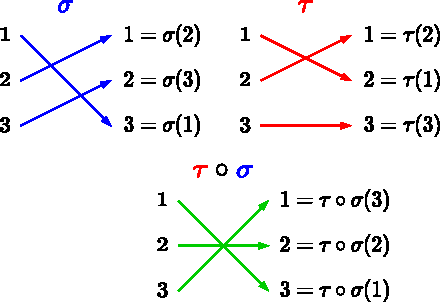
\includegraphics[keepaspectratio, width=0.55\linewidth]{determinant2.pdf}
\end{figure}
\end{frame}

\begin{frame}{置換に関する性質}
\begin{itemize}
  \item 恒等置換を, $\iota$とかく.
  $$\iota = \left\{ 1, 2, 3 \right\} \to \left\{ 1, 2, 3 \right\}$$
  \item $\sigma^{-1} \sigma = \sigma \sigma^{-1} = \iota, \quad \sgn(\tau \sigma) = \sgn(\tau) \sgn(\sigma)$
  \item $\sgn(\iota) = 1, \quad \sgn(\sigma^{-1}) = \sgn(\sigma)$
  \item $\vb{A} = \mqty(a_{ij})$を行列, $\sigma$を置換としたとき,
  $$a_{\sigma^{-1}(1) 1} a_{\sigma^{-1}(2) 2} \cdots a_{\sigma^{-1}(n) n}
    = a_{1 \sigma(1)} a_{2 \sigma(2)} \cdots a_{n \sigma(n)}$$
  \item $\sigma = \left\{ 1, 2, 3 \right\} \to \left\{ 2, 3, 1 \right\}$とする.
  $\sigma^{-1} = \left\{ 2, 3, 1 \right\} \to \left\{ 1, 2, 3 \right\}$となる.
  \begin{align*}
    a_{\sigma^{-1}(1) 1} a_{\sigma^{-1}(2) 2} a_{\sigma^{-1}(3) 3}
      &= a_{31} a_{12} a_{23} = a_{12} a_{23} a_{31} \\
      &= a_{1 \sigma(1)} a_{2 \sigma(2)} a_{3 \sigma(3)}
  \end{align*}
\end{itemize}
\end{frame}

\begin{frame}{置換に関する性質}
\begin{itemize}
  \item $\vb{A} = \mqty(a_{ij})$を行列, $\sigma$を置換としたとき,
  $$a_{\sigma^{-1}(1) 1} a_{\sigma^{-1}(2) 2} \cdots a_{\sigma^{-1}(n) n}
    = a_{1 \sigma(1)} a_{2 \sigma(2)} \cdots a_{n \sigma(n)}$$
  \item $\sigma = \left\{ 1, 2, 3 \right\} \to \left\{ 2, 3, 1 \right\}$とする.
  $\sigma^{-1} = \left\{ 2, 3, 1 \right\} \to \left\{ 1, 2, 3 \right\}$となる.
  \begin{align*}
    a_{\sigma^{-1}(1) 1} a_{\sigma^{-1}(2) 2} a_{\sigma^{-1}(3) 3}
      &= a_{1 \sigma(1)} a_{2 \sigma(2)} a_{3 \sigma(3)}
  \end{align*}
\end{itemize}

\begin{figure}
  \centering
  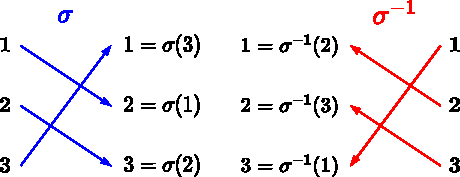
\includegraphics[keepaspectratio, width=0.65\linewidth]{determinant1.pdf}
\end{figure}
\end{frame}

\begin{frame}{転置の行列式}
\begin{block}{転置の行列式}
  $$\det(\vb{A}^\top) = \det(\vb{A})$$
\end{block}

\begin{itemize}
  \item 行列式の定義から,
  \begin{align*}
    \det(\vb{A}) &= \sum_{\sigma \in S_n} \sgn(\sigma)
      a_{1 \sigma(1)} a_{2 \sigma(2)} \cdots a_{n \sigma(n)} \\
    \det(\vb{A}^\top) &= \sum_{\tau \in S_n} \sgn(\tau)
      \left( \vb{A}^\top \right)_{1 \tau(1)} \left( \vb{A}^\top \right)_{2 \tau(2)}
      \left( \vb{A}^\top \right)_{n \tau(n)} \\
      &= \sum_{\tau \in S_n} \sgn(\tau)
        a_{\tau(1) 1} a_{\tau(2) 2} \cdots a_{\tau(n) n}
  \end{align*}
\end{itemize}
\end{frame}

\begin{frame}{転置の行列式}
\begin{itemize}
  \item 行列式の定義から,
  \begin{align*}
    \det(\vb{A}) &= \sum_{\sigma \in S_n} \sgn(\sigma)
      a_{1 \sigma(1)} a_{2 \sigma(2)} \cdots a_{n \sigma(n)} \\
    \det(\vb{A}^\top) &= \sum_{\tau \in S_n} \sgn(\tau)
      a_{\tau(1) 1} a_{\tau(2) 2} \cdots a_{\tau(n) n}
  \end{align*}
  \item $\sigma^{-1}$について総和を取ることは, $\sigma$について総和を取ることと同じだから, 
  $\tau = \sigma^{-1}$とする.
  \item $\tau = \sigma^{-1}$とおくと, $\sgn(\tau) = \sgn(\sigma^{-1}) = \sgn(\sigma)$であり,
  以下が成り立つので, $\det(\vb{A}) = \det(\vb{A}^\top)$.
  \begin{align*}
    a_{\tau(1) 1} a_{\tau(2) 2} \cdots a_{\tau(n) n}
      &= a_{\sigma^{-1}(1) 1} a_{\sigma^{-1}(2) 2} \cdots a_{\sigma^{-1}(n) n} \\
      &= a_{1 \sigma(1)} a_{2 \sigma(2)} \cdots a_{n \sigma(n)}
  \end{align*}
\end{itemize}
\end{frame}

\begin{frame}{対角行列の行列式}
\begin{block}{対角行列の行列式}
  $n$次の対角行列があるとする.
  行列式は, 対角成分$\lambda_1, \ldots, \lambda_n$の積となる.
  $$\det(\mqty(\dmat{\lambda_1, \lambda_2, \ddots, \lambda_n})) = \prod_i \lambda_i$$
\end{block}

\begin{itemize}
  \item 行列式の定義において, 恒等置換$\iota$に対応する項だけが残る:
  \begin{align*}
    \det(\vb{A}) &= \sum_{\sigma \in S_n} \sgn(\sigma)
      a_{1 \sigma(1)} a_{2 \sigma(2)} \cdots a_{n \sigma(n)} \\
      &= a_{11} a_{22} \cdots a_{n n}
      = \prod_i \lambda_i
  \end{align*}
\end{itemize}
\end{frame}

\begin{frame}{上三角行列, 下三角行列の行列式}
\begin{block}{上三角行列, 下三角行列の行列式}
  $n \times n$の上三角, 下三角行列があるとする.
  行列式は, 対角成分$\lambda_1, \ldots, \lambda_n$の積となる.
  \begin{align*}
    \det\left( \mqty(\lambda_1 & * & \cdots & * \\
      & \lambda_2 & \ddots & \vdots \\
      & & \ddots & * \\
      & & & \lambda_n) \right) &= \prod_i \lambda_i \\
    \det\left( \mqty(\lambda_1 \\ * & \lambda_2 \\
      \vdots & \ddots & \ddots \\
      * & \cdots & * & \lambda_n) \right) &= \prod_i \lambda_i
  \end{align*}
\end{block}
\end{frame}

\begin{frame}{上三角行列, 下三角行列の逆行列の行列式}
\begin{block}{上三角行列, 下三角行列の逆行列の行列式}
  元の対角成分の逆数$\lambda_1^{-1}, \ldots, \lambda_n^{-1}$の積となる.
  \begin{align*}
    \det\left( \mqty(\lambda_1 & * & \cdots & * \\
      & \lambda_2 & \ddots & \vdots \\
      & & \ddots & * \\
      & & & \lambda_n)^{-1} \right) &= \prod_i \lambda_i^{-1} \\
    \det\left( \mqty(\lambda_1 \\ * & \lambda_2 \\
      \vdots & \ddots & \ddots \\
      * & \cdots & * & \lambda_n)^{-1} \right) &= \prod_i \lambda_i^{-1}
  \end{align*}
\end{block}
\end{frame}

\begin{frame}{列の線形変換, 列の入れ替え, 行列のスカラー倍}
\begin{block}{列の線形変換, 列の入れ替え}
  列を入れ替えると, 行列式の符号が反転する.
  \begin{gather*}
    \det(\mqty(\vb{a}_1, \ldots, \lambda \vb{a}_i + \mu \vb{b}_i, \ldots, \vb{a}_n))
      = \lambda \det(\mqty(\vb{a}_1, \ldots, \vb{a}_i, \ldots, \vb{a}_n)) \\
        + \mu \det(\mqty(\vb{a}_1, \ldots, \vb{b}_i, \ldots, \vb{a}_n)) \\
    \det(\mqty(\vb{a}_1, \ldots, \vb{a}_i, \ldots, \vb{a}_j, \ldots, \vb{a}_n))
      = -\det(\mqty(\vb{a}_1, \ldots, \vb{a}_j, \ldots, \vb{a}_i, \ldots, \vb{a}_n))
  \end{gather*}
\end{block}

\begin{block}{行列のスカラー倍}
  行列を$c$倍すると, 行列式は$c^n$倍になる.
  $$\det(c \vb{A}) = c^n \det(\vb{A})$$
\end{block}

\begin{itemize}
  \item $\det(\vb{A}^\top) = \det(\vb{A})$であるから, 列だけでなく, 行についても同様のことがいえる.
\end{itemize}
\end{frame}

\begin{frame}{列の線形変換, 列のスカラー倍}
\begin{block}{同じ列を含むとき}
  同じ列ベクトルを2箇所に含むとき, 行列式は$0$となる.
  $$\det(\mqty(\vb{a}_1, \ldots, \vb{a}_i, \ldots, \vb{a}_i, \ldots, \vb{a}_n)) = 0$$
\end{block}

\begin{block}{列のスカラー倍}
  列を$c$倍すると, 行列式は$c$倍になる.
  $$\det(\mqty(\vb{a}_1, \ldots, c \vb{a}_i, \ldots, \vb{a}_n))
    = c \det(\mqty(\vb{a}_1, \ldots, \vb{a}_i, \ldots, \vb{a}_n))$$
  $i$列目に, $j$列目の$c$倍を足しても ($i \neq j$), 行列式は変わらない.
  \begin{align*}
    \small
    \det(\mqty(\vb{a}_1, \ldots, \vb{a}_i + c \vb{a}_j, \ldots, \vb{a}_j, \ldots, \vb{a}_n))
      = \det(\mqty(\vb{a}_1, \ldots, \vb{a}_i, \ldots, \vb{a}_j, \ldots, \vb{a}_n))
  \end{align*}
\end{block}

\begin{itemize}
  \item $\det(\vb{A}^\top) = \det(\vb{A})$であるから, 列だけでなく, 行についても同様のことがいえる.
\end{itemize}
\end{frame}

\begin{frame}{行列積, 行列の累乗, 逆行列}
\begin{block}{行列積, 行列の累乗の行列式}
  \begin{gather*}
    \det(\vb{A} \vb{B}) = \det(\vb{A}) \det(\vb{B}) \\
    \det(\vb{A}^n) = \det(\vb{A})^n
  \end{gather*}
\end{block}

\begin{block}{逆行列の行列式}
  $$\det(\vb{A}^{-1}) = \frac{1}{\det(\vb{A})}$$
\end{block}

\begin{itemize}
  \item 以下の2つの式から分かる.
  \begin{gather*}
    \det(\vb{A} \vb{A}^{-1}) = \det(\vb{A}) \det(\vb{A}^{-1}) \\
    \det(\vb{A} \vb{A}^{-1}) = \det(\vb{I}) = 1
  \end{gather*}
\end{itemize}
\end{frame}

\begin{frame}{固有値と固有ベクトル}
\begin{itemize}
  \item $\vb{A}$を, $n$次正方行列とする.
  \item 以下を満たすような$\lambda$を, $\vb{A}$の\textcolor{red}{固有値}という.
  \item また$\vb{x}$を, 固有値$\lambda$に対する\textcolor{red}{固有ベクトル}という.
  $$\vb{A} \vb{x} = \lambda \vb{x}$$
  \item 上式は, $\det(\lambda \vb{I} - \vb{A}) = 0$と同値である (詳細は省略).
  \item $\det(\lambda \vb{I} - \vb{A}) = 0$の左辺を展開すれば, $\lambda$に関する$n$次式となる:
  $$(\lambda - \lambda_1) (\lambda - \lambda_2) \cdots (\lambda - \lambda_n) = 0$$
  \item 上式は, 固有多項式という. 重複を許せば, 固有値は$n$個ある.
  \item $\vb{A}$が正則であれば (逆行列があれば), $\lambda_i \neq 0$.
\end{itemize}
\end{frame}

\begin{frame}{固有値と固有ベクトル}
\begin{itemize}
  \item $\vb{A}$の逆行列の固有値は, $\vb{A}$の固有値の逆数$\lambda_1^{-1}, \ldots, \lambda_n^{-1}$である.
  \item また, $\vb{A}$の逆行列は, $\vb{A}$と共通の固有ベクトルをもつ.
  \item $\vb{A}$の固有値は以下を満たす.
  $$\vb{A} \vb{x} = \lambda \vb{x}$$
  \item これを式変形すればよい ($\vb{A}$は正則なので, $\lambda \neq 0$).
  $$\vb{x} = \lambda \vb{A}^{-1} \vb{x}
    \qquad \to \qquad \lambda^{-1} \vb{x} = \vb{A}^{-1} \vb{x}$$
\end{itemize}
\end{frame}

\begin{frame}{固有値と行列式}
\begin{block}{固有値と行列式}
  $\vb{A}$を, $n$次正方行列とする.
  $\vb{A}$の固有値$\lambda_1, \ldots, \lambda_n$の積は, $\vb{A}$の行列式となる.
  $$\det(\vb{A}) = \prod_{i = 1}^n \lambda_i$$
\end{block}

\begin{itemize}
  \item 以下の固有多項式について, $\lambda = 0$とする.
  $$\det(\lambda \vb{I} - \vb{A}) = (\lambda - \lambda_1) (\lambda - \lambda_2) \cdots (\lambda - \lambda_n)$$
  \item 左辺は, $\det(-\vb{A}) = (-1)^n \det(\vb{A})$.
  \item 右辺は, $\prod_i (-\lambda_i) = (-1)^n \prod_i \lambda_i$.
\end{itemize}
\end{frame}

\begin{frame}{固有値と行列式}
\begin{block}{固有値と行列式}
  $\vb{A}$を, $n$次正方行列とする.
  $\vb{A}$の固有値の逆数$\lambda_1^{-1}, \ldots, \lambda_n^{-1}$の積は, $\vb{A}^{-1}$の行列式となる.
  $$\det(\vb{A}^{-1}) = \prod_{i = 1}^n \lambda_i^{-1}$$
\end{block}

\begin{itemize}
  \item $\det(\vb{A}^{-1}) = \det(\vb{A})^{-1}$と, $\det(\vb{A}) = \prod_i \lambda_i$から分かる.
\end{itemize}
\end{frame}

\begin{frame}{ブロック上三角行列, 下三角行列の行列式}
\begin{block}{ブロック上三角行列, 下三角行列の行列式}
  \begin{align*}
    \det\left( \mqty(\vb{I} & \vb{X} \\ \vb{0} & \vb{I}) \right) &= 1, \quad
    \det\left( \mqty(\vb{I} & \vb{0} \\ \vb{X} & \vb{I}) \right) = 1 \\
    \det\left( \mqty(\vb{A} & \vb{B} \\ \vb{0} & \vb{D}) \right)
      &= \det(\vb{A}) \det(\vb{D}) \\
    \det\left( \mqty(\vb{A} & \vb{0} \\ \vb{C} & \vb{D}) \right)
      &= \det(\vb{A}) \det(\vb{D}) \\
    \det\left( \mqty(\vb{A} & \vb{B} \\ \vb{B} & \vb{A}) \right)
      &= \det(\vb{A} + \vb{B}) \det(\vb{A} - \vb{B})
  \end{align*}
\end{block}

\begin{itemize}
  \item 証明は省略.
\end{itemize}
\end{frame}

\begin{frame}{ブロック対角行列の行列式}
\begin{block}{ブロック対角行列の行列式}
  \begin{align*}
    \det\left( \mqty(\dmat{\vb{A}_1, \vb{A}_2, \ddots, \vb{A}_n}) \right)
      &= \det(\vb{A}_1) \det(\vb{A}_2) \cdots \det(\vb{A}_n) \\
    \det\left( \mqty(\dmat{\vb{A}_1, \vb{A}_2, \ddots, \vb{A}_n})^{-1} \right)
      &= \det(\vb{A}_1)^{-1} \det(\vb{A}_2)^{-1} \cdots \det(\vb{A}_n)^{-1}
  \end{align*}
\end{block}
\end{frame}

\begin{frame}{ブロック行列の行列式}
\begin{block}{ブロック行列の行列式}
  \begin{align*}
    \det\left( \mqty(\vb{A} & \vb{B} \\ \vb{C} & \vb{D}) \right)
      &= \det(\vb{A}) \det(\vb{D} - \vb{C} \vb{A}^{-1} \vb{B}) & \text{$\vb{A}$が正則} \\
    \det\left( \mqty(\vb{A} & \vb{B} \\ \vb{C} & \vb{D}) \right)
      &= \det(\vb{D}) \det(\vb{A} - \vb{B} \vb{D}^{-1} \vb{C}) & \text{$\vb{D}$が正則}
  \end{align*}
\end{block}

\begin{itemize}
  \item シューア補行列による表現から導出できる (上側).
  \begin{gather*}
    \mqty(\vb{A} & \vb{B} \\ \vb{C} & \vb{D})
      = \mqty(\vb{I} & \vb{0} \\ \vb{C} \vb{A}^{-1} & \vb{I})
        \mqty(\dmat[\vb{0}]{\vb{A}, \vb{D} - \vb{C} \vb{A}^{-1} \vb{B}})
        \mqty(\vb{I} & \vb{A}^{-1} \vb{B} \\ \vb{0} & \vb{I})
  \end{gather*}
  \item 3つの行列の行列式の積を求める.
  \item 最初と最後の行列の行列式は$1$である.
\end{itemize}
\end{frame}

\begin{frame}{ブロック行列の行列式}
\begin{block}{Weinstein-Aronszajn Identity}
  $\vb{A}$を$m \times n$, $\vb{B}$を$n \times m$の行列とする.
  $$\det(\vb{I}_m + \vb{A} \vb{B}) = \det(\vb{I}_n + \vb{B} \vb{A})$$
  $\vb{a}, \vb{b}$が$m$次ベクトルであるとき,
  $$\det(\vb{I}_m + \vb{a} \vb{b}^\top) = 1 + \vb{b}^\top \vb{a}$$
\end{block}

\begin{itemize}
  \item 先ほどの式において ($\vb{I}_m$, $\vb{I}_n$は正則であるので),
  \begin{align*}
    \det\left( \mqty(\vb{I}_m & -\vb{A} \\ \vb{B} & \vb{I}_n) \right)
      &= \det(\vb{I}_m) \det(\vb{I}_n + \vb{B} \vb{I}_m^{-1} \vb{A})
      = \det(\vb{I}_n + \vb{B} \vb{A}) \\
      &= \det(\vb{I}_n) \det(\vb{I}_m + \vb{A} \vb{I}_n^{-1} \vb{B})
      = \det(\vb{I}_m + \vb{A} \vb{B})
  \end{align*}
\end{itemize}
\end{frame}

\begin{frame}{余因子展開}
\begin{block}{余因子展開}
  $\vb{A}$を, $n$次正方行列とする. 各$i$行目と$j$列目について,
  \begin{align*}
    \det(\vb{A}) &= a_{i1} \Delta_{i1} + a_{i2} \Delta_{i2} + \cdots + a_{in} \Delta_{in}
      = \sum_j a_{ij} \Delta_{ij} \\
    \det(\vb{A}) &= a_{1j} \Delta_{1j} + a_{2j} \Delta_{2j} + \cdots + a_{nj} \Delta_{nj}
      = \sum_i a_{ij} \Delta_{ij}
  \end{align*}
\end{block}

\begin{itemize}
  \item 上式の$\Delta_{ij}$は, $\vb{A}$の\textcolor{red}{$(i, j)$余因子} (Cofactor) とよぶ.
  $$\Delta_{ij} = (-1)^{i + j} \det(\tilde{\vb{A}}_{ij})$$
  \item $\tilde{\vb{A}}_{ij}$は, $\vb{A}$から$i$行目と$j$列目を取り除いた, $n - 1$次行列である.
  \item $\Delta_{ij}$は, $i$行目と$j$行目の成分には依存しない.
\end{itemize}
\end{frame}

\begin{frame}{余因子展開}
\begin{block}{余因子展開}
  $\vb{A}$を, $n$次正方行列とする.
  $\Delta_{ij}$を$\vb{A}$の$(i, j)$余因子とする.
  \begin{align*}
    a_{i1} \Delta_{k1} + a_{i2} \Delta_{k2} + \cdots + a_{in} \Delta_{kn}
      &= \left\{ \begin{array}{ll} \det(\vb{A}) & i = k \\ 0 & \text{Otherwise} \end{array} \right. \\
    a_{1j} \Delta_{1k} + a_{2j} \Delta_{2k} + \cdots + a_{nj} \Delta_{nk}
      &= \left\{ \begin{array}{ll} \det(\vb{A}) & j = k \\ 0 & \text{Otherwise} \end{array} \right.
  \end{align*}
\end{block}
\end{frame}

\begin{frame}{余因子行列}
\begin{block}{余因子行列}
  $\vb{A}$を, $n$次行列とする.
  $\vb{A}$の$(i, j)$余因子$\Delta_{ij}$を並べた行列$\adj \vb{A}$を, $\vb{A}$の余因子行列という.
  $$\adj \vb{A} = \mqty(\Delta_{11} & \Delta_{21} & \cdots & \Delta_{n1} \\
    \Delta_{12} & \Delta_{22} & \cdots & \Delta_{n2} \\
    \vdots & \vdots & \ddots & \vdots \\
    \Delta_{1n} & \Delta_{2n} & \cdots & \Delta_{nn})$$
\end{block}

\begin{itemize}
  \item $\adj \vb{A}$の\textcolor{red}{$(i, j)$成分は, $(j, i)$余因子$\Delta_{ji}$}となる.
\end{itemize}
\end{frame}

\begin{frame}{余因子行列, 行列式, 逆行列}
\begin{block}{余因子行列, 行列式, 逆行列}
  $\vb{A}$の余因子行列$\adj \vb{A}$, 行列式$\det(\vb{A})$, 逆行列$\vb{A}^{-1}$について,
  $$\left( \adj \vb{A} \right) \vb{A} = \vb{A} \left( \adj \vb{A} \right)
    = \left( \det(\vb{A}) \right) \vb{I}$$
  $$\vb{A}^{-1} = \frac{1}{\det(\vb{A})} \adj \vb{A}$$
\end{block}
\end{frame}

\section{トレース}

\begin{frame}{行列のトレース}
\begin{itemize}
  \item $\vb{A}$を, $n$次正方行列とする.
  \item $\vb{A}$の対角成分$a_{ii}$の和を, $\vb{A}$の\textcolor{red}{トレース}とよぶ.
  \item トレースを, $\tr(\vb{A})$とかく.
  $$\tr(\vb{A}) = \sum_i a_{ii}$$
  \item 歪対称行列 ($\vb{A}^\top = -\vb{A}$) の対角成分は$0$なので, トレースは$0$.
  \item 単位行列 $\vb{I}_n$ のトレースは$n$.
\end{itemize}
\end{frame}

\begin{frame}{行列の和, 転置とトレース}
\begin{block}{行列の和, 転置とトレース}
  \begin{gather*}
    \tr(\vb{A} + \vb{B}) = \tr(\vb{A}) + \tr(\vb{B}) \\
    \tr(\vb{A}^\top) = \tr(\vb{A})
  \end{gather*}
\end{block}

\begin{itemize}
  \item トレースの定義から, 以下のように確認できる.
  \begin{align*}
    \tr(\vb{A} + \vb{B}) &= \sum_i \left( \vb{A} + \vb{B} \right)_{ii}
      = \sum_i \left( a_{ii} + b_{ii} \right) = \sum_i a_{ii} + \sum_i b_{ii} \\
      &= \tr(\vb{A}) + \tr(\vb{B}) \\
    \tr(\vb{A}^\top) &= \sum_i \left( \vb{A}^\top \right)_{ii}
      = \sum_i a_{ii} = \tr(\vb{A})
  \end{align*}
\end{itemize}
\end{frame}

\begin{frame}{行列の積とトレース}
\begin{block}{行列の積とトレース}
  $$\tr(\vb{A} \vb{B}) = \tr(\vb{B} \vb{A})$$
\end{block}

\begin{itemize}
  \item トレースの定義から, 以下のように確認できる.
  \begin{align*}
    \tr(\vb{A} \vb{B}) &= \sum_i \left( \vb{A} \vb{B} \right)_{ii}
      = \sum_i \sum_k a_{ik} b_{ki}
      = \sum_k \sum_i b_{ki} a_{ik} \\
      &= \sum_k \left( \vb{B} \vb{A} \right)_{kk}
      = \tr(\vb{B} \vb{A})
  \end{align*}
\end{itemize}
\end{frame}

\begin{frame}{トレースの循環性}
\begin{block}{トレースの循環性}
  $$\tr(\vb{A} \vb{B} \vb{C}) = \tr(\vb{B} \vb{C} \vb{A}) = \tr(\vb{C} \vb{A} \vb{B})$$
  $$\tr(\vb{X}^{-1} \vb{A} \vb{X}) = \tr(\vb{A})$$
\end{block}

\begin{itemize}
  \item トレースの定義から, 以下のように確認できる.
  \begin{align*}
    \tr(\vb{A} \vb{B} \vb{C}) &= \sum_i \left( \vb{A} \vb{B} \vb{C} \right)_{ii}
      = \sum_i \sum_k \sum_l a_{ik} b_{kl} c_{li} \\
      &= \sum_k \sum_l \sum_i b_{kl} c_{li} a_{ik} = \tr(\vb{B} \vb{C} \vb{A}) \\
      &= \sum_l \sum_i \sum_k c_{li} a_{ik} b_{kl} = \tr(\vb{C} \vb{A} \vb{B})
  \end{align*}
  \item たらい回しのような公式である.
\end{itemize}
\end{frame}

\begin{frame}{行列, ベクトル積とトレース}
\begin{block}{行列, ベクトル積とトレース}
  $\vb{A}$を, $n$次正方行列, $\vb{b}, \vb{c}$を$n$次ベクトルとする.
  $$\tr(\vb{A} \vb{b} \vb{c}^\top) = \vb{c}^\top \vb{A} \vb{b}$$
  $$\tr(\vb{b} \vb{c}^\top) = \vb{c}^\top \vb{b}$$
\end{block}

\begin{itemize}
  \item $\vb{b}, \vb{c}$がベクトルで, 上のような形であれば, 順序を入れ替えることでトレース$\tr$を除去できる.
\end{itemize}
\end{frame}

\begin{frame}{固有値とトレース}
\begin{block}{固有値とトレース}
  $\vb{A}$を, $n$次正方行列とする.
  $\vb{A}$の固有値$\lambda_1, \ldots, \lambda_n$の和は, $\vb{A}$のトレースとなる.
  $$\tr(\vb{A}) = \sum_i \lambda_i$$
\end{block}

\begin{itemize}
  \item 以下の固有多項式について, $\lambda^{n - 1}$の係数を考える.
  $$\det(\lambda \vb{I} - \vb{A}) = (\lambda - \lambda_1) (\lambda - \lambda_2) \cdots (\lambda - \lambda_n)$$
  \item 左辺は, $-\tr(\vb{A})$.
  \begin{itemize}
    \item $\det(\lambda \vb{I} - \vb{A})$には, $\left( \lambda - a_{11} \right)
    \left( \lambda - a_{22} \right) \cdots \left( \lambda - a_{nn} \right)$という項が現れる.
    \item $\lambda^{n - 1}$の係数は, $-(a_{11} + a_{22} + \cdots + a_{nn})$となる.
  \end{itemize}
  \item 右辺は, $-\sum_i \lambda_i$.
\end{itemize}
\end{frame}

\begin{frame}{逆行列とトレース}
\begin{block}{逆行列とトレース}
  $\vb{A}$を, $n$次正方行列とする.
  $\vb{A}$の逆行列のトレースは, $\vb{A}$の固有値$\lambda_1, \ldots, \lambda_n$の逆数の和となる.
  $$\tr(\vb{A}^{-1}) = \sum_i \lambda_i^{-1}$$
\end{block}

\begin{itemize}
  \item $\vb{A}$は, ユニタリ行列$\vb{P}$により, $\vb{P}^{-1} \vb{A} \vb{P}$と三角化できる (後述).
  \item $\vb{P}^{-1} \vb{A} \vb{P}$の対角成分は, $\vb{A}$の固有値$\lambda_1, \ldots, \lambda_n$である.
  \item $\vb{P}^{-1} \vb{A} \vb{P}$の逆行列も三角行列で, $\lambda_1^{-1}, \ldots, \lambda_n^{-1}$を対角成分にもつので,
  \begin{align*}
    \tr(\left( \vb{P}^{-1} \vb{A} \vb{P} \right)^{-1}) &= \sum_i \lambda_i^{-1} \\
      &= \tr(\vb{P}^{-1} \vb{A}^{-1} \vb{P}) = \tr(\vb{A}^{-1} \vb{P} \vb{P}^{-1}) = \tr(\vb{A}^{-1})
  \end{align*}
\end{itemize}
\end{frame}

\begin{frame}{対角行列のトレース}
\begin{block}{対角行列のトレース}
  $\vb{A} = \diag(a_1, a_2, \ldots, a_n)$を$n$次対角行列とする.
  $\vb{A}, \vb{A}^{-1}$のトレースは, 次のようになる.
  \begin{align*}
    \tr(\vb{A}) &= \tr\left( \mqty(\dmat{a_1, \ddots, a_n}) \right) = \sum_i a_i \\
    \tr(\vb{A}^{-1}) &= \tr\left( \mqty(\dmat{a_1^{-1}, \ddots, a_n^{-1}}) \right) = \sum_i a_i^{-1}
  \end{align*}
\end{block}
\end{frame}

\begin{frame}{上三角行列, 下三角行列の逆行列のトレース}
\begin{block}{上三角行列, 下三角行列の逆行列のトレース}
  元の対角成分の逆数$\lambda_1^{-1}, \ldots, \lambda_n^{-1}$の和となる.
  \begin{align*}
    \tr\left( \mqty(\lambda_1 & * & \cdots & * \\
      & \lambda_2 & \ddots & \vdots \\
      & & \ddots & * \\
      & & & \lambda_n)^{-1} \right) &= \sum_i \lambda_i^{-1} \\
    \tr\left( \mqty(\lambda_1 \\ * & \lambda_2 \\
      \vdots & \ddots & \ddots \\
      * & \cdots & * & \lambda_n)^{-1} \right) &= \sum_i \lambda_i^{-1}
  \end{align*}
\end{block}
\end{frame}

\begin{frame}{ブロック行列のトレース}
\begin{block}{ブロック行列のトレース}
  $$\tr\left( \mqty(\vb{A}_1 & * & \cdots & * \\
    * & \vb{A}_2 & \ddots & \vdots \\
    \vdots & \ddots & \ddots & \vdots \\
    * & \cdots & * & \vb{A}_n) \right) = \sum_i \tr(\vb{A}_i)$$
\end{block}
\end{frame}

\begin{frame}{固有値, 対角化, 三角化に関するまとめ}
\begin{itemize}
  \item $\vb{A}$を, $n$次正方行列とする.
  \item $\vb{A}$に$n$個の線形独立な固有ベクトルがあれば, それを並べた行列$\vb{P}$で,
  $\vb{P}^{-1} \vb{A} \vb{P}$と対角化できる (対角成分は$\vb{A}$の固有値).
  \item 任意の$\vb{A}$は, ユニタリ行列$\vb{P}$で, $\vb{P}^{-1} \vb{A} \vb{P}$と\textcolor{red}{三角化}できる
  (上三角行列, 対角成分は$\vb{A}$の固有値).
  \item $\vb{A}$が正規行列 ($\vb{A} \vb{A}^\mathrm{H} = \vb{A}^\mathrm{H} \vb{A}$) なら,
  ユニタリ行列で対角化できる.
  \begin{itemize}
    \item $\vb{A}^\mathrm{H}$は, $\vb{A}$の共役転置.
    \item 正規行列: ユニタリ行列 ($\vb{A} \vb{A}^\mathrm{H} = \vb{I}$),
    エルミート行列 ($\vb{A}^\mathrm{H} = \vb{A}$), 歪エルミート行列 ($\vb{A}^\mathrm{H} = -\vb{A}$),
    直交行列 ($\vb{A} \vb{A}^\top = \vb{I}$), 対称行列 ($\vb{A}^\top = \vb{A}$), 歪対称行列 ($\vb{A}^\top = -\vb{A}$).
  \end{itemize}
  \item $\vb{A}$が実対称行列なら, 直交行列で対角化できる.
  \item エルミート行列と対称行列の固有値は, 全て実数である.
\end{itemize}
\end{frame}

% ヤコビの公式
% 微分

\end{document}
